% !TeX root = ../main.tex
\section{Capteur thermistance (SEMI833-ET)}

\subsection{Mesure manuelle de la température ambiante}
\label{subsec:ntc_ambiante}

La thermistance CTN (SEMI833-ET) présente une résistance nominale de \qty{103.6}{\kilo\ohm} à \qty{20}{\degreeCelsius}. 
À l'aide du multimètre de table de précision Keysight 34460A réglé en configuration deux fils (résolution maximale 6½ digits), la résistance mesurée aux bornes du capteur à l'air libre dans le laboratoire est :
\begin{equation}
    R_{\text{mes}} = \qty{97.20}{\kilo\ohm}
\end{equation}

D'après la table de référence de la datasheet constructeur, la thermistance présente dans cette zone de température une variation moyenne de résistance par degré :
\begin{itemize}[leftmargin=1.2cm]
    \item Pente locale à \qty{20}{\degreeCelsius} : $p_{20} = \qty{4.70}{\kilo\ohm\per\degreeCelsius}$ ;
    \item Pente locale à \qty{25}{\degreeCelsius} : $p_{25} = \qty{3.63}{\kilo\ohm\per\degreeCelsius}$ ;
    \item Pente moyenne sur l'intervalle $[20\,^\circ\text{C}\,;\,25\,^\circ\text{C}]$ : $p_{\text{moy}} = \frac{4.70 + 3.63}{2} = \qty{4.165}{\kilo\ohm\per\degreeCelsius}$.
\end{itemize}

Comme la résistance mesurée (\qty{97.20}{\kilo\ohm}) est inférieure à la valeur nominale à \qty{20}{\degreeCelsius} (\qty{103.60}{\kilo\ohm}), la température ambiante est supérieure à \qty{20}{\degreeCelsius} (caractéristique CTN à coefficient de température négatif) :
\begin{equation}
    T_{\text{amb}} = 20 + \frac{R_{\text{nom, } 20^\circ\text{C}} - R_{\text{mes}}}{p_{\text{moy}}} = 20 + \frac{103.60 - 97.20}{4.165} = 20 + 1.54 = \qty{21.54}{\degreeCelsius}
\end{equation}

\subsubsection*{Estimation de l'incertitude sur la mesure manuelle NTC}
Selon la fiche constructeur de la perle SEMI833-ET, la tolérance d'interchangeabilité de fabrication sans étalonnage individuel est garantie à $\pm \qty{0.8}{\degreeCelsius}$ autour de la température ambiante. Compte tenu de la précision métrologique du multimètre Keysight 34460A (incertitude de lecture inférieure à $\pm \qty{0.02}{\kilo\ohm}$ sur la gamme $\qty{100}{\kilo\ohm}$, induisant un écart thermique inférieur à $\qty{0.005}{\degreeCelsius}$), l'incertitude sur la température ambiante est totalement dominée par la dispersion technologique du capteur :
\begin{equation}
    T_{\text{amb, NTC}} = \mathbf{\qty{21.54 \pm 0.80}{\degreeCelsius}} \quad \text{avec } u(T_{\text{amb, NTC}}) = \qty{0.80}{\degreeCelsius}
\end{equation}

\subsection{Mesure de la résistance par pont diviseur et auto-échauffement}
\label{subsec:ntc_pont}

Afin d'adapter le signal à la carte d'acquisition analogique (National Instruments PCIe-6321), un pont diviseur de tension est constitué avec une résistance fixe de valeur étalonnée $R = \qty{462.35}{\kilo\ohm}$ (valeur nominale \qty{470}{\kilo\ohm}) alimenté sous une tension continue $V_{CC} = \qty{14.00}{\volt}$ via l'alimentation stabilisée de table GW Instek GPD-3303S.

\subsubsection*{Formule inverse de calcul de $R_{NTC}$}
La tension mesurée aux bornes de la CTN $U_{NTC}$ s'exprime par la relation du pont diviseur :
\begin{equation}
    U_{NTC} = V_{CC} \cdot \frac{R_{NTC}}{R + R_{NTC}}
\end{equation}
En isolant $R_{NTC}$, on obtient la relation inverse programmée dans le sous-VI LabVIEW :
\begin{equation}
    R_{NTC} = \frac{R \cdot U_{NTC}}{V_{CC} - U_{NTC}}
    \label{eq:formule_rntc}
\end{equation}

\subsubsection*{Calcul de l'auto-échauffement}
À température ambiante ($R_{NTC} \approx \qty{97.2}{\kilo\ohm}$ et $R = \qty{462.35}{\kilo\ohm}$), la tension aux bornes de la thermistance vaut :
\begin{equation}
    U_{NTC} = 14.00 \cdot \frac{97.20}{462.35 + 97.20} \approx \qty{2.43}{\volt}
\end{equation}
La puissance électrique dissipée par effet Joule dans la perle thermistance est :
\begin{equation}
    P = \frac{U_{NTC}^2}{R_{NTC}} = \frac{(2.43)^2}{97.2 \cdot 10^3} \approx \qty{6.08e-5}{\watt} \approx \qty{0.061}{\milli\watt}
\end{equation}
La perle SEMI833-ET possède un coefficient de dissipation thermique en air calme typique de l'ordre de $\delta \approx \qty{0.7}{\milli\watt\per\degreeCelsius}$. L'auto-échauffement théorique induit par la mesure s'élève donc à :
\begin{equation}
    \Delta T = \frac{P}{\delta} \approx \frac{\qty{0.061}{\milli\watt}}{\qty{0.7}{\milli\watt\per\degreeCelsius}} \approx \mathbf{\qty{0.09}{\degreeCelsius}}
\end{equation}
Cet échauffement interne de moins d'un dixième de degré reste très faible et négligeable devant la tolérance générale du capteur ($\pm \qty{0.8}{\degreeCelsius}$), ce qui valide le dimensionnement de la résistance série $R \approx \qty{470}{\kilo\ohm}$.

\subsection{Chaîne d'acquisition et conversion sous LabVIEW}
\label{subsec:ntc_labview}

L'acquisition automatisée du signal du pont diviseur est implémentée dans l'environnement LabVIEW avec la carte d'acquisition multifonction National Instruments PCIe-6321 :
\begin{itemize}[leftmargin=1.2cm]
    \item \textbf{Configuration différentielle de la voie analogique :} La tension $U_{NTC}$ est mesurée en mode différentiel (\textit{Differential}) afin de rejeter les tensions de mode commun et les parasites électromagnétiques induits par les boucles de masse du laboratoire.
    \item \textbf{Cadencement temporel :} La boucle de lecture logicielle est cadencée à une période d'échantillonnage de \qty{20}{\milli\second} (soit une fréquence d'échantillonnage de \qty{50}{\hertz}).
    \item \textbf{Calcul de température en deux étages :}
    \begin{enumerate}
        \item Le premier sous-VI calcule la valeur instantanée de la résistance $R_{NTC}$ à partir de la tension acquise $U_{NTC}$ en appliquant la formule inverse du pont diviseur~\eqref{eq:formule_rntc}.
        \item Le second sous-VI traduit la résistance en température au moyen du VI standard LabVIEW « Scaling and Mapping » configuré en mode \textit{Interpolation}. La table de conversion discrète nominale est chargée directement à partir du fichier constructeur \texttt{Echelle\_SEMI833.lvm}.
    \end{enumerate}
\end{itemize}
Le signal ainsi étalonné est visualisé en temps réel sur un graphe déroulant avant enregistrement pour les essais sous flux d'air chaud.

\subsection{Mesures en flux d'air chaud et suréchantillonnage}
\label{subsec:ntc_oversampling}

Les séries temporelles de mesure de température acquises en plaçant la CTN dans le flux d'air chaud du sèche-cheveux à pleine puissance sont présentées et comparées à la figure~\ref{fig:diff_over_normal}. Deux modes d'acquisition ont été exécutés durant environ \qty{10}{\second} :
\begin{enumerate}[leftmargin=1.2cm]
    \item \textbf{Mode standard (Section 1.4) :} lecture échantillon par échantillon cadencée à \qty{20}{\milli\second} par temporisation logicielle ($N = 520$ points) ;
    \item \textbf{Mode suréchantillonné (Section 1.5) :} lecture matérielle cadencée par paquets de $100$ échantillons moyennés arithmétiquement sous LabVIEW avant affichage ($N = 375$ points).
\end{enumerate}

\begin{figure}[H]
    \centering
    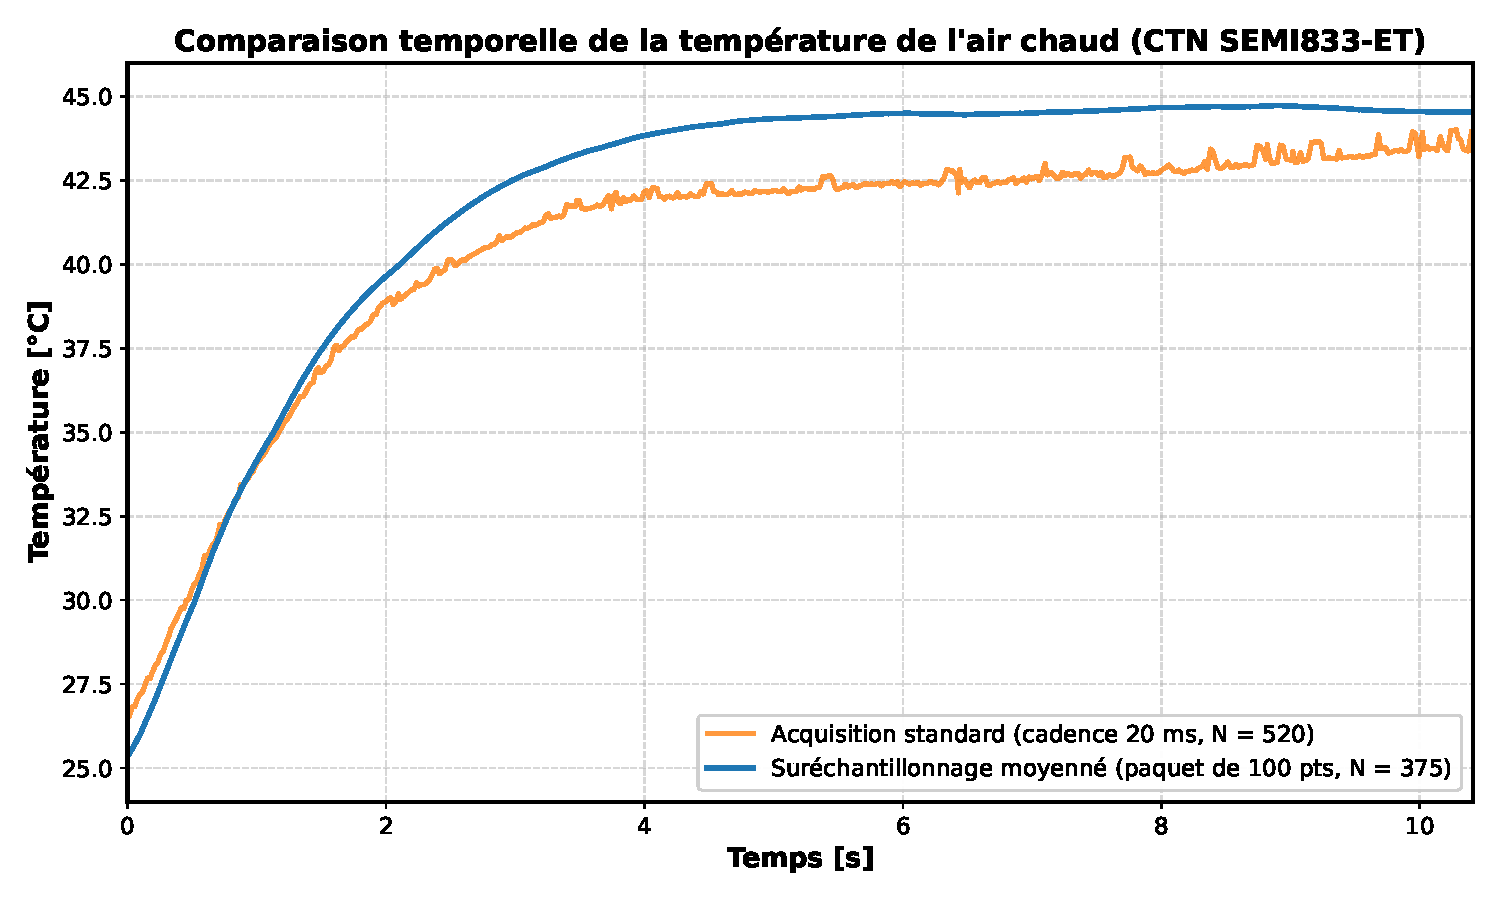
\includegraphics[width=0.92\textwidth]{assets/graphs/comparaison_ntc_oversampling.pdf}
    \caption{Comparaison temporelle de la température de l'air en sortie du sèche-cheveux : série standard cadencée à \qty{20}{\milli\second} ($N = 520$) et série suréchantillonnée moyennant $100$ échantillons par point ($N = 375$). Les labels d'axes respectent les normes TechMes avec les unités entre crochets.}
    \label{fig:diff_over_normal}
\end{figure}

\subsubsection*{Analyse statistique quantitative des deux séries}
Le calcul des grandeurs statistiques (moyenne arithmétique $\bar{T}$, écart-type d'échantillon $\sigma$ et incertitude-type sur la moyenne $u(\bar{T}) = \sigma / \sqrt{N}$) sur l'intégralité de l'enregistrement donne :
\begin{itemize}[leftmargin=1.2cm]
    \item \textbf{Série standard ($N = 520$) :}
    \begin{align}
        \bar{T}_{\text{norm}} &= \qty{40.56}{\degreeCelsius} \\
        \sigma_{\text{norm}} &= \qty{3.96}{\degreeCelsius} \\
        u(\bar{T}_{\text{norm}}) &= \frac{\sigma_{\text{norm}}}{\sqrt{N}} = \frac{3.96}{\sqrt{520}} = \qty{0.17}{\degreeCelsius} \quad \implies \quad \bar{T}_{\text{norm}} = \mathbf{\qty{40.56 \pm 0.17}{\degreeCelsius}}
    \end{align}
    \item \textbf{Série avec suréchantillonnage ($N = 375$) :}
    \begin{align}
        \bar{T}_{\text{over}} &= \qty{41.90}{\degreeCelsius} \\
        \sigma_{\text{over}} &= \qty{4.75}{\degreeCelsius} \\
        u(\bar{T}_{\text{over}}) &= \frac{\sigma_{\text{over}}}{\sqrt{N}} = \frac{4.75}{\sqrt{375}} = \qty{0.25}{\degreeCelsius} \quad \implies \quad \bar{T}_{\text{over}} = \mathbf{\qty{41.90 \pm 0.25}{\degreeCelsius}}
    \end{align}
\end{itemize}

\noindent
\textbf{Analyse du régime stabilisé (après montée thermique) :} \\
Lors des premières \qty{0.5}{\second} de chaque manipulation, le capteur subit une phase transitoire d'échauffement rapide depuis la température ambiante ($\approx \qty{25}{\degreeCelsius}$ à \qty{26}{\degreeCelsius}) jusqu'au flux stabilisé du sèche-cheveux. Si l'on restreint l'évaluation statistique au palier stationnaire (exclusion des 23 premiers points transitoires), on relève :
\begin{itemize}[leftmargin=1.2cm]
    \item Série standard stabilisée ($N = 497$) : $\bar{T}_{\text{norm, stab}} = \qty{41.13}{\degreeCelsius}$, $\sigma_{\text{norm, stab}} = \qty{2.98}{\degreeCelsius}$ et $u(\bar{T}) = \qty{0.13}{\degreeCelsius}$ ;
    \item Série suréchantillonnée stabilisée ($N = 352$) : $\bar{T}_{\text{over, stab}} = \qty{42.83}{\degreeCelsius}$, $\sigma_{\text{over, stab}} = \qty{3.15}{\degreeCelsius}$ et $u(\bar{T}) = \qty{0.17}{\degreeCelsius}$.
\end{itemize}

\subsubsection*{Discussion physique du suréchantillonnage et répétabilité expérimentale}
Le suréchantillonnage (\textit{oversampling}) avec moyennage synchrone apporte un filtrage passe-bas numérique rigoureux : le bruit blanc de conversion analogique-numérique (bruit de quantification et bruit thermique de l'étage ADC de la carte NI PCIe-6321) est atténué théoriquement d'un facteur $\sqrt{n} = \sqrt{100} = 10$, procurant un gain effectif de $\approx 3.32$ bits de résolution.

Cependant, les écarts-types observés sur le signal stabilisé ($\sigma \approx \qty{3}{\degreeCelsius}$) restent comparables entre les deux séries. Cette observation confirme que la variance du signal n'est pas limitée par le bruit électronique de la chaîne d'acquisition, mais par la physique même de l'écoulement aéraulique : le jet d'un sèche-cheveux présente des turbulences thermiques chaotiques et des tourbillons convectifs intrinsèques de forte amplitude.

Par ailleurs, on remarque sur la figure~\ref{fig:diff_over_normal} que les deux courbes ne sont pas rigoureusement superposées en température moyenne (décalage systématique de $\approx \qty{1.34}{\degreeCelsius}$ sur la moyenne globale et $\approx \qty{1.70}{\degreeCelsius}$ sur le palier stabilisé). Cette différence s'explique de manière prépondérante par l'absence de répétabilité géométrique parfaite de la manipulation : le sèche-cheveux et la perle du capteur étaient tenus manuellement par les opérateurs, sans dispositif de fixation rigide ni guidage mécanique. Les inévitables micro-mouvements de la main et de légères variations de position, de distance et d'orientation angulaire dans le cône de gradient thermique du flux d'air chaud entre les deux séries successives modifient légèrement l'apport convectif reçu par le capteur. Le suréchantillonnage élimine le bruit de haute fréquence de l'électronique sans pouvoir effacer les fluctuations physiques et les biais de manipulation du milieu en mouvement.
